
\section{Pre-Trained Models}
This section describes the results obtained using different pre-trained architecture and strategies\footnote{The data augmentation strategy is always used since we have very little data}. The pre-trained networks here tested are:
\begin{itemize}
\item VGG16
\item ResNet50V2
\item ResNet101V2
\item InceptionV3
\end{itemize}
 
\subsection{VGG16}
VGG16\ref{fig:vgg16} is a convolutional neural network model proposed by Simonyan et al., with several 3x3 convolutional layers in cascade occasionally interleaved with 2x2 max-pooling layers forming the so called \textit{blocks}. Developed for the ILSVRC2014 challenge, it was able to achieve a top-5 accuracy of 92.7 on ImageNet.
\begin{figure}[H]
	\centering
	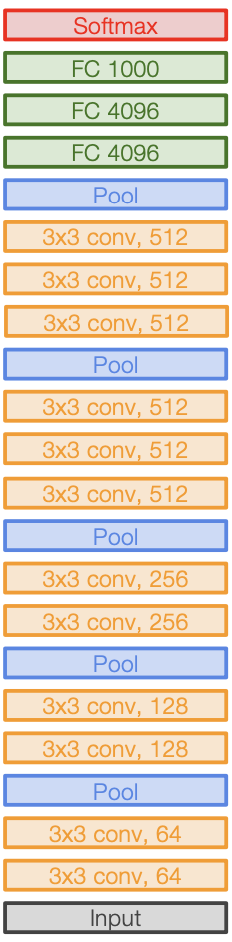
\includegraphics[height=0.7\textwidth]{img/vgg16/vgg16.png}
	\caption{VGG16 Architecture}
	\label{fig:vgg16}
\end{figure}

\subsubsection{Test 1: Classical VGG16 (Feature Extraction)}
The original VGG16 comes with a couple of 4096 FC layers followed by 1000 softmax neurons, which is alright for ImageNet but definitely oversized for our purpose. Hence, the convolutional base is left as it is, and the fully-connected block is replaced by the a shrunk version with only 256 neurons per layer, followed by our prediction layer made of 11 neurons\ref{fig:vgg16fe1}.

\begin{figure}[H]
	\centering
	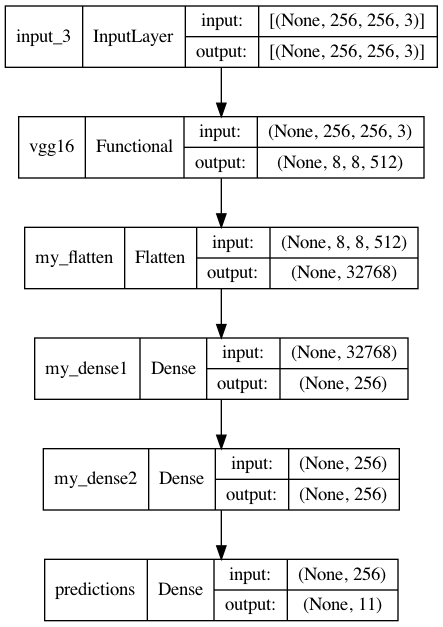
\includegraphics[height=0.5\textwidth]{img/vgg16/vgg16fe1.png}
	\caption{Our Feature Extraction Network}
	\label{fig:vgg16fe1}
\end{figure}


\noindent The result obtained, using RMSprop as optimizer, are:

\medskip

\begin{tabular}{ |p{2cm}|p{2cm}|p{2cm}|p{2cm}|p{2cm}|  }
\hline
\multicolumn{5}{|c|}{Feature Extraction} \\
\hline
\textbf{Epoch stopped} & \textbf{Validation Accuracy} & \textbf{Testing Accuracy} & \textbf{Validation Loss} & \textbf{Testing Loss} \\
\hline
12 & 0.7409 & 0.7057 & 5.1959 & 5.7\\
\hline
\end{tabular}

\medskip

 \noindent The network begin to overfit very fast, hence some regularization methods are needed.


\begin{figure}[H]
	\begin{subfigure}{0.5\textwidth}
		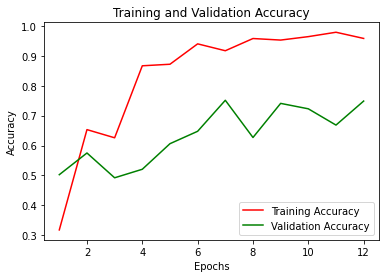
\includegraphics[width=0.9\linewidth]{img/vgg16/vgg16fe1acc.png} 
		\caption{Simple VGG16 Feature Extraction Accuracy}
		\label{fig:vgg16fe1acc}
	\end{subfigure}
	\begin{subfigure}{0.5\textwidth}
		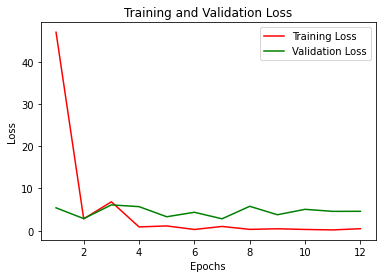
\includegraphics[width=0.9\linewidth]{img/vgg16/vgg16fe1loss.png}
		\caption{Simple VGG16 Feature Extraction Loss}
		\label{fig:vgg16fe1loss}
	\end{subfigure}
\end{figure}

\subsubsection{Test 2: Adding Dropout to Test 1}
We have two possible positions to use the dropout layer in our network and they are after each 256-dense layer, but we decided to use just one layer at the end of the second 256-Dense layer (\textit{my\_dense1}) as shown in Figure\ref{fig:vgg16fe2}. We didn't use a dropout layer between the two 256-dense layers, since this type of architecture led to worst performance, this mainly because we would have less units to fully train our topic-specific network.
\begin{figure}[H]
	\centering
	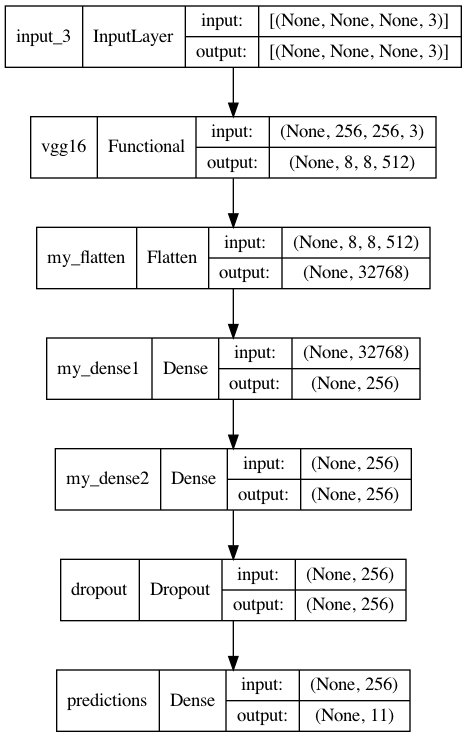
\includegraphics[height=0.45\textwidth]{img/vgg16/vgg16fe2.png}
	\caption{Our Feature Extraction Network + Dropout}
	\label{fig:vgg16fe2}
\end{figure}
  

\noindent The result obtained, using RMSprop as optimizer, are:

\medskip

\begin{tabular}{ |p{2cm}|p{2cm}|p{2cm}|p{2cm}|p{2cm}|  }
\hline
\multicolumn{5}{|c|}{Feature Extraction w/ dropout} \\
\hline
\textbf{Epoch stopped} & \textbf{Validation Accuracy} & \textbf{Testing Accuracy} & \textbf{Validation Loss} & \textbf{Testing Loss} \\
\hline
25 & 0.7306 & 0.7195 & 3.0616 & 3.0035\\
\hline
\end{tabular}

\medskip

\begin{figure}[H]
	\begin{subfigure}{0.5\textwidth}
		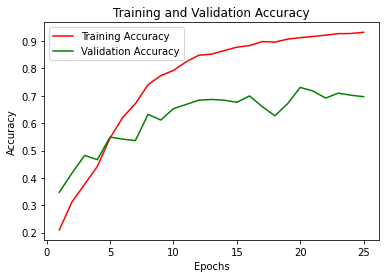
\includegraphics[width=0.9\linewidth]{img/vgg16/vgg16fe2acc.png} 
		\caption{Test 2 Accuracy}
		\label{fig:vgg16fe2acc}
	\end{subfigure}
	\begin{subfigure}{0.5\textwidth}
		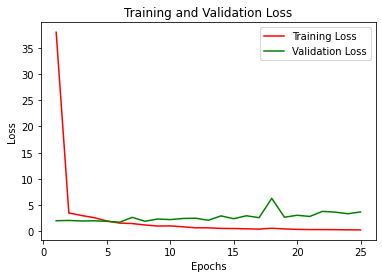
\includegraphics[width=0.9\linewidth]{img/vgg16/vgg16fe2loss.png}
		\caption{Test 2 Loss}
		\label{fig:vgg16fe2oss}
	\end{subfigure}
\end{figure}

\noindent As expected, dropout mitigated the magnitude of overfitting, however our network perform slightly worst (now the validation accuracy is 0.73 and before was 0.74) than without the dropout layer.


\subsubsection{Test 3: Finetuning One Convolutional Layer}
Using the model defined in test 1, the 3rd Conv2D layer in the 5th block is un-fronzen and the network is trained. The result obtained using RMSprop as optimizer are the following:

 
 \medskip

\begin{tabular}{ |p{2cm}|p{2cm}|p{2cm}|p{2cm}|p{2cm}|  }
\hline
\multicolumn{5}{|c|}{Finetuning one convolutional layer} \\
\hline
\textbf{Epoch stopped} & \textbf{Validation Accuracy} & \textbf{Testing Accuracy} & \textbf{Validation Loss} & \textbf{Testing Loss} \\
\hline
28 & 0.7202 & 0.6253 & 2.3687 & 8.1807\\
\hline
\end{tabular}

\medskip

\begin{figure}[H]
	\begin{subfigure}{0.5\textwidth}
		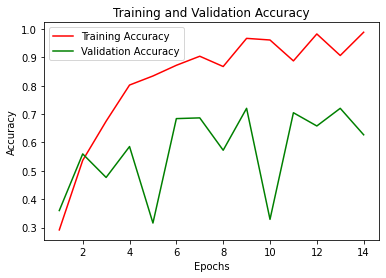
\includegraphics[width=0.9\linewidth]{img/vgg16/vgg16ft1acc.png} 
		\caption{Test 3 Accuracy}
		\label{fig:vgg16ft1acc}
	\end{subfigure}
	\begin{subfigure}{0.5\textwidth}
		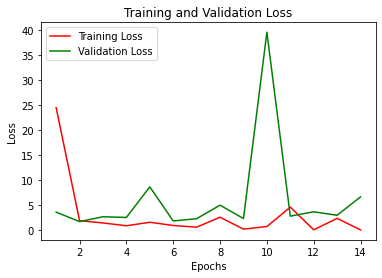
\includegraphics[width=0.9\linewidth]{img/vgg16/vgg16ft1loss.png}
		\caption{Test 3 Loss}
		\label{fig:vgg16ft1loss}
	\end{subfigure}
\end{figure}


Again the performance are worst than in test one, but looking at the graphs it can be seen that not only our network overfitted very fast, but it forms also few fang-shaped changes in direction. 






\subsubsection{Test 4: test 3 with dropout and different optimizer}
To overcome the previous problems, the overfitting and the strange shape behavior, in this test we opt to use \textbf{Adam} as an optimizer, changing its default learning rate (i.e., 0.001) to 0.0001 in order to slowly learn and hoping to have a smoother accuracy and loss functions.

 
 \medskip

\begin{tabular}{ |p{2cm}|p{2cm}|p{2cm}|p{2cm}|p{2cm}|  }
\hline
\multicolumn{5}{|c|}{Finetuning one conv layer w/ dropout and Adam} \\
\hline
\textbf{Epoch stopped} & \textbf{Validation Accuracy} & \textbf{Testing Accuracy} & \textbf{Validation Loss} & \textbf{Testing Loss} \\
\hline
28 & 0.7358 & 0.7218 & 0.9871 & 1.1792\\
\hline
\end{tabular}

\medskip

\begin{figure}[H]
	\begin{subfigure}{0.5\textwidth}
		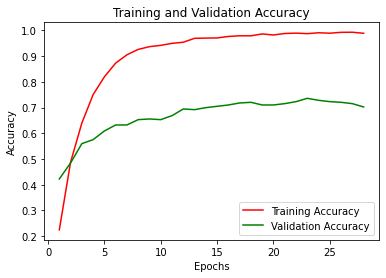
\includegraphics[width=0.9\linewidth]{img/vgg16/vgg16ft1dropacc.png} 
		\caption{Test 4 Accuracy}
		\label{fig:vgg16ft1dropacc}
	\end{subfigure}
	\begin{subfigure}{0.5\textwidth}
		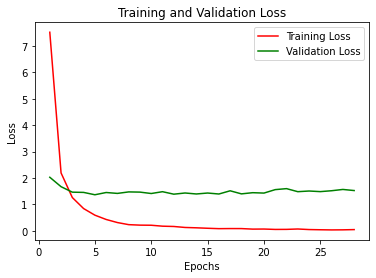
\includegraphics[width=0.9\linewidth]{img/vgg16/vgg16ft1droploss.png}
		\caption{Test 4 Loss}
		\label{fig:vgg16ft1droploss}
	\end{subfigure}
\end{figure}


\noindent Adding dropout and a different optimizer with a little learning rate, we finally obtained what we were aiming. Anyway, the result is now comparable to the test 1, however now we our using a more complex network which is not good if the results are the same.

However we can still do something, the training accuracy increases very rapidly even if dropout is applied. To decrease this effect in test 6 we use weight regularization techniques.



\subsubsection{Test 5: Finetuning Two Convolutional Layers}
This test is basically test 4, but finetuning the last two convolutional layers of VGG16.

 \medskip

\begin{tabular}{ |p{2cm}|p{2cm}|p{2cm}|p{2cm}|p{2cm}|  }
\hline
\multicolumn{5}{|c|}{Finetuning two convolutional layers} \\
\hline
\textbf{Epoch stopped} & \textbf{Validation Accuracy} & \textbf{Testing Accuracy} & \textbf{Validation Loss} & \textbf{Testing Loss} \\
\hline
22 & 0.7280 & 0.7379 & 1.4253 & 1.2589\\
\hline
\end{tabular}

\medskip

\begin{figure}[H]
	\begin{subfigure}{0.5\textwidth}
		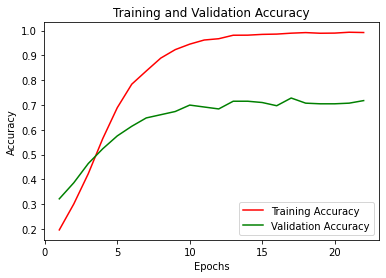
\includegraphics[width=0.9\linewidth]{img/vgg16/vgg16ft2dropacc.png} 
		\caption{Test 5 Accuracy}
		\label{fig:vgg16ft2dropacc}
	\end{subfigure}
	\begin{subfigure}{0.5\textwidth}
		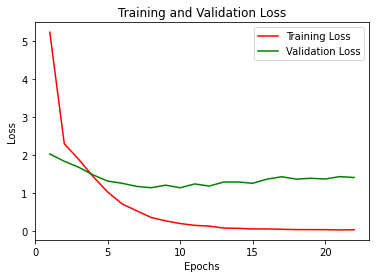
\includegraphics[width=0.9\linewidth]{img/vgg16/vgg16ft2droploss.png}
		\caption{Test 5 Loss}
		\label{fig:vgg16ft2droploss}
	\end{subfigure}
\end{figure}


Following the approach used in the previous test we obtained also here more smoothed graphs, but the performance is little lower than before. The problem here is that we are propagating to the second layer in block 5 gradients that are not really improvements of the ones set by the \textit{imagenet} default configuration.






\subsubsection{Test 6: Finetuning One Convolutional Layer and Weights Regularization}
In this paragraph we exploited the conclusion mentioned in test 4, introducing here \textit{L1\_L2 weight regularization} on the one convolutional layer finetuned network.


\medskip

\begin{tabular}{ |p{2cm}|p{2cm}|p{2cm}|p{2cm}|p{2cm}|  }
\hline
\multicolumn{5}{|c|}{Finetuning one conv layer and weights regularization} \\
\hline
\textbf{Epoch stopped} & \textbf{Validation Accuracy} & \textbf{Testing Accuracy} & \textbf{Validation Loss} & \textbf{Testing Loss} \\
\hline
22& 0.7487 & 0.7471 & 21.5590 & 9.8097\\
\hline
\end{tabular}

\medskip

\begin{figure}[H]
	\begin{subfigure}{0.5\textwidth}
		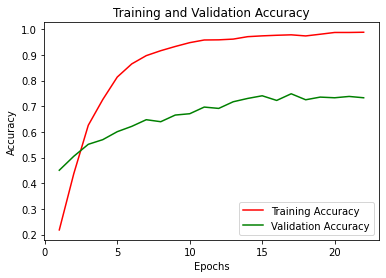
\includegraphics[width=0.9\linewidth]{img/vgg16/vgg16ft1dropregacc.png} 
		\caption{Test 6 Accuracy}
		\label{fig:vgg16ft1dropregacc}
	\end{subfigure}
	\begin{subfigure}{0.5\textwidth}
		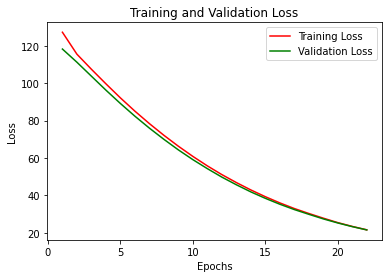
\includegraphics[width=0.9\linewidth]{img/vgg16/vgg16ft1dropregloss.png}
		\caption{Test 6 Loss}
		\label{fig:vgg16ft1dropregloss}
	\end{subfigure}
\end{figure}

The shapes of the graphs are more or less the same of the two had in test 4, the only things that changes are the values of the losses which are here higher and more curvilinear due to the weight regularization approach used. Anyway, this heavy regularization helped us to surpass the result in test 1, not by much but it is an improvement that, maybe, can be exploited finetuning more. Following this lead, in the next paragraph we use weight regularization with two convolutional layers finetuned.






\subsubsection{Test 7: Finetuning Two Convolutional Layers and Weights Regularization}
Following the good result obtained in test 6, in this paragraph we add, to the network used in test 5, \textit{L1\_L2 weight regularization}.

 \medskip

\begin{tabular}{ |p{2cm}|p{2cm}|p{2cm}|p{2cm}|p{2cm}|  }
\hline
\multicolumn{5}{|c|}{Finetuning two conv layers and weights regularization} \\
\hline
\textbf{Epoch stopped} & \textbf{Validation Accuracy} & \textbf{Testing Accuracy} & \textbf{Validation Loss} & \textbf{Testing Loss} \\
\hline
25 & 0.7694 & 0.7494 & 15.6742 & 9.8097\\
\hline
\end{tabular}

\medskip


\begin{figure}[H]
	\begin{subfigure}{0.5\textwidth}
		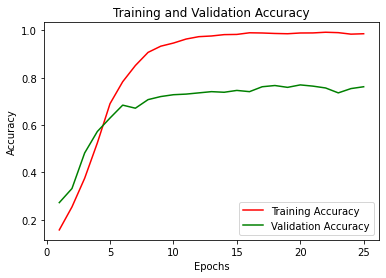
\includegraphics[width=0.9\linewidth]{img/vgg16/vgg16ft2dropregacc.png} 
		\caption{Test 7 Accuracy}
		\label{fig:vgg16ft2dropregacc}
	\end{subfigure}
	\begin{subfigure}{0.5\textwidth}
		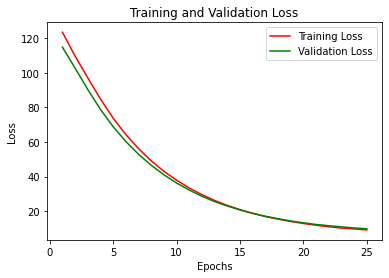
\includegraphics[width=0.9\linewidth]{img/vgg16/vgg16ft2dropregloss.png}
		\caption{Test 7 Loss}
		\label{fig:vgg16ft2dropregloss}
	\end{subfigure}
\end{figure}

Even if the increase the flexibility of our network finetuning more layers, as hoped, we achieved a better accuracy which is also the best obtained so far.




\subsubsection{Test 8: Genetic Algorithm for Hyper-parameters and Architecture Optimization}





\subsection{ResNet50V2}
ResNet stands for Residual Network. It is an innovative neural network that was first introduced by Kaiming He, Xiangyu Zhang, Shaoqing Ren, and Jian Sun in their 2015 computer vision research paper titled "Deep Residual Learning for Image Recognition". This model was immensely successful, as can be ascertained from the fact that its ensemble won the top position at the ILSVRC 2015 classification competition with an error of only 3.57\%. Additionally, it also came first in the ImageNet detection, ImageNet localization, COCO detection, and COCO segmentation in the ILSVRC \& COCO competitions of 2015.



\subsubsection{Test 1: Classical ResNet50V2 (Feature Extraction)}
The original ResNet50 comes with a GlobalAveragePooling2D and a prediction layer soon after. In this test we used the same approach, resizing the prediction layer to the number of classes we have.

\noindent The results obtained after training are:
\medskip

\begin{tabular}{ |p{2cm}|p{2cm}|p{2cm}|p{2cm}|p{2cm}|  }
\hline
\multicolumn{5}{|c|}{Feature Extraction} \\
\hline
\textbf{Epoch stopped} & \textbf{Validation Accuracy} & \textbf{Testing Accuracy} & \textbf{Validation Loss} & \textbf{Testing Loss} \\
\hline
39 & 0.4430 & 0.3241 & 5.3733 & 6.8513\\
\hline
\end{tabular}

\begin{figure}[H]
	\begin{subfigure}{0.5\textwidth}
		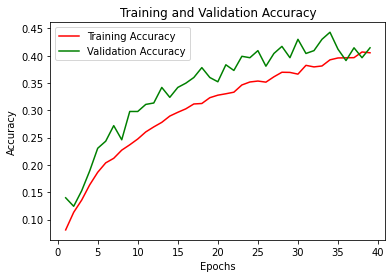
\includegraphics[width=0.9\linewidth]{img/resnet50v2/resnet50acc.png} 
		\caption{Simple ResNet50V2 Feature Extraction Accuracy}
	\end{subfigure}
	\begin{subfigure}{0.5\textwidth}
		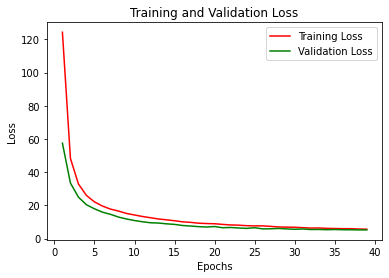
\includegraphics[width=0.9\linewidth]{img/resnet50v2/resnet50loss.png}
		\caption{Simple ResNet50V2 Feature Extraction Loss}
	\end{subfigure}
\end{figure}

The network poorly performed compered with the results obtained using VGG16. This can be explained since the \textit{imagenet dataset} is not specialized in distinguish paintings' artists, thus the frozen weights of our networks are very far to be the ones we need. To overcome this problem we can fine tune or add more layers after the \textit{GlobalAveragePooling2D} layer.

Another problem can be notice looking at the accuracy plot, the training accuracy is less than the validation accuracy. To understand this issue, it is important to consider the difference of the number of images in the training and validation set. The validation set is made of about few hundreds of pictures against the few thousands of the training set, the latter may involve, with greater probability, paintings being part of a different period of the artists (e.g., the example shown in Image\ref{fig:picasso}), which can lead to a worst accuracy.


\subsubsection{Test 2: Finetuning 1 block}
ResNet50V2 is made of multiple big blocks (i.e., 5) so called \textit{conv} in the model. These blocks are made of sub-blocks connected by each other by an add layer which connects the processed input (e.g., processed by Conv2D, Padding, Pooling, BatchNormalization) and the residual input\footnote{Sometimes the residual is downsampled using a max pooling layer, this is done in order to match the actual size of the feature map obtained at that level of the network.}. We finetuned considering this under-blocks, hence in this paragraph we finetuned the \textit{conv5\_block3}.

\medskip

\begin{tabular}{ |p{2cm}|p{2cm}|p{2cm}|p{2cm}|p{2cm}|  }
\hline
\multicolumn{5}{|c|}{Finetuning 1 block} \\
\hline
\textbf{Epoch stopped} & \textbf{Validation Accuracy} & \textbf{Testing Accuracy} & \textbf{Validation Loss} & \textbf{Testing Loss} \\
\hline
18 & 0.6399 & 0.5793 & 1.2453 & 1.7916\\
\hline
\end{tabular}

\begin{figure}[H]
	\begin{subfigure}{0.5\textwidth}
		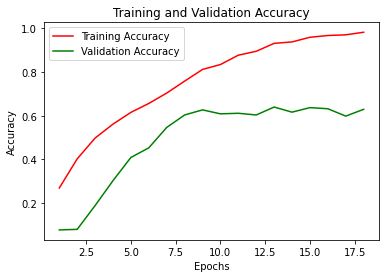
\includegraphics[width=0.9\linewidth]{img/resnet50v2/resnet50finetuned1acc.png} 
		\caption{ResNet50V2 Test 2 Accuracy}
		\label{fig:resnet50finetuned1acc}
	\end{subfigure}
	\begin{subfigure}{0.5\textwidth}
		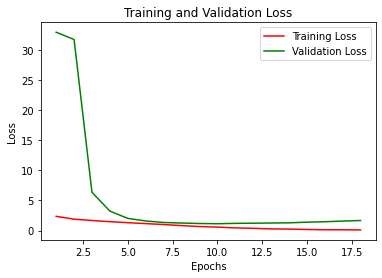
\includegraphics[width=0.9\linewidth]{img/resnet50v2/resnet50finetuned1loss.png}
		\caption{ResNet50V2 Test 2 Loss}
		\label{fig:resnet50finetuned1loss}
	\end{subfigure}
\end{figure}

\noindent As expected, the network has definitely reach a more satisfactory result. Also the behaviors of the curves now is more reasonable. 



\subsubsection{Test 3: Finetuning 2 blocks}
Since finetuning a block led to better results, the next step we did was to tuning also the previous sub-block, thus starting to tuning from \textit{conv5\_block2}.

\medskip

\begin{tabular}{ |p{2cm}|p{2cm}|p{2cm}|p{2cm}|p{2cm}|  }
\hline
\multicolumn{5}{|c|}{Finetuning 2 blocks} \\
\hline
\textbf{Epoch stopped} & \textbf{Validation Accuracy} & \textbf{Testing Accuracy} & \textbf{Validation Loss} & \textbf{Testing Loss} \\
\hline
20 & 0.6477 & 0.6092 & 1.5918 & 1.7734\\
\hline
\end{tabular}

\begin{figure}[H]
	\begin{subfigure}{0.5\textwidth}
		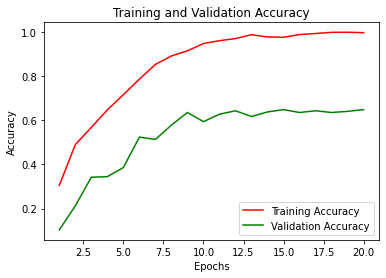
\includegraphics[width=0.9\linewidth]{img/resnet50v2/resnet50finetuned2acc.png} 
		\caption{ResNet50V2 Test 3 Accuracy}
		\label{fig:resnet50finetuned2acc}
	\end{subfigure}
	\begin{subfigure}{0.5\textwidth}
		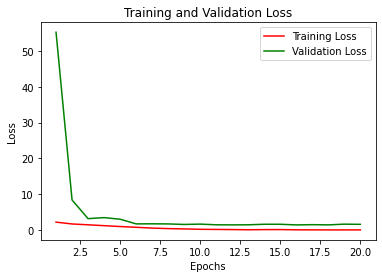
\includegraphics[width=0.9\linewidth]{img/resnet50v2/resnet50finetuned2loss.png}
		\caption{ResNet50V2 Test 3 Loss}
		\label{fig:resnet50finetuned2loss}
	\end{subfigure}
\end{figure}

This results proves that our idea of finetuning was good since the network improved a little. Anyway, finetuning more can be risky since the computational power and time needed can be very high and becoming unbearable to the limits imposed by Colab. Thus, we tried to improved (without satisfaction, as the nexts to paragraphs describe) our network adding dense layers between our \textit{GlobalAveragePooling2D} and our prediction layer, following the structure used in the VGG16 study.



\subsubsection{Test 4: Finetuning with One Block and Adding Two Dense layers}
Here we took the same approach of test 3, but adding two dense layers followed by a dropout layer (as used in figure\ref{fig:vgg16fe2}).

\medskip

\begin{tabular}{ |p{2cm}|p{2cm}|p{2cm}|p{2cm}|p{2cm}|  }
\hline
\multicolumn{5}{|c|}{Finetuning one block and dense layers} \\
\hline
\textbf{Epoch stopped} & \textbf{Validation Accuracy} & \textbf{Testing Accuracy} & \textbf{Validation Loss} & \textbf{Testing Loss} \\
\hline
20 & 0.6736 & 0.6368 & 1.6655 & 1.7734\\
\hline
\end{tabular}

\begin{figure}[H]
	\begin{subfigure}{0.5\textwidth}
		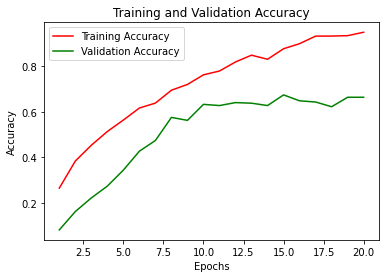
\includegraphics[width=0.9\linewidth]{img/resnet50v2/resnet50finetuned1denseacc.png} 
		\caption{ResNet50V2 Test 4 Accuracy}
		\label{fig:resnet50finetuned1denseacc}
	\end{subfigure}
	\begin{subfigure}{0.5\textwidth}
		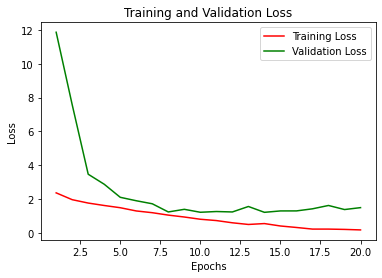
\includegraphics[width=0.9\linewidth]{img/resnet50v2/resnet50finetuned1denseloss.png}
		\caption{ResNet50V2 Test 4 Loss}
		\label{fig:resnet50finetuned1denseloss}
	\end{subfigure}
\end{figure}

Enlarging in this way the network resulted in better performance. This can be because the dense layers before the softmax can better exploit the information of the \textit{GlobalAveragePooling2D}, keeping the problem for more time to a higher dimensionally than the one used for prediction.


\subsubsection{Test 5: Finetuning with Two Blocks and Adding Two Dense layers}
In this paragraph we did the same thing done in test 4, but finetuning two blocks as in test 3.

\medskip

\begin{tabular}{ |p{2cm}|p{2cm}|p{2cm}|p{2cm}|p{2cm}|  }
\hline
\multicolumn{5}{|c|}{Finetuning two blocks and dense layers} \\
\hline
\textbf{Epoch stopped} & \textbf{Validation Accuracy} & \textbf{Testing Accuracy} & \textbf{Validation Loss} & \textbf{Testing Loss} \\
\hline
17 & 0.6373 & 0.5954 & 1.6404 & 2.1089\\
\hline
\end{tabular}

\begin{figure}[H]
	\begin{subfigure}{0.5\textwidth}
		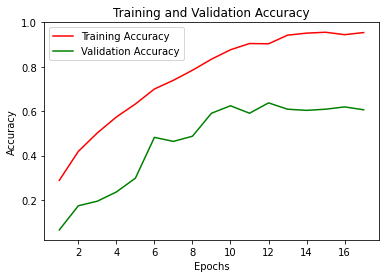
\includegraphics[width=0.9\linewidth]{img/resnet50v2/resnet50finetuned2denseacc.png} 
		\caption{ResNet50V2 Test 5 Accuracy}
		\label{fig:resnet50finetuned2denseacc}
	\end{subfigure}
	\begin{subfigure}{0.5\textwidth}
		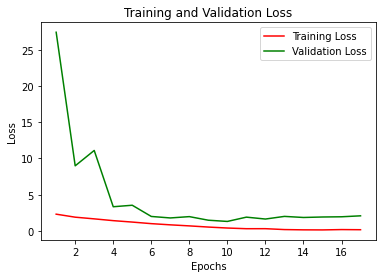
\includegraphics[width=0.9\linewidth]{img/resnet50v2/resnet50finetuned2denseloss.png}
		\caption{ResNet50V2 Test 5 Loss}
		\label{fig:resnet50finetuned2denseloss}
	\end{subfigure}
\end{figure}


Unfortunately, finetuning this much with these additional layers led to worst performance. Perhaps, this is due to backpropagation, which changed the weights (which are 9M, against the 14M that are not trainable) to a not-optimal solution. Anyway, this result is also too poor compared to test 3, which without having the newly added dense layers still perform better.







\subsection{ResNet101V2}
ResNet101 was implemented as one of the model used in the ensemble method cited in the ResNet50V2 introduction. ResNet101 is an extension of ResNet50 that goes deeper reaching 101 layers in depth, simply adding more convolutional 'sub'-blocks in the blocks\footnote{Referring to the notation used before, we intend as a sub-block a block between two adds.}. ResNet101 proved to be slightly more accurate than ResNet50.\footnote{It is not only additional network used in the ensemble method, an extension of it was also used, ResNet152. This model is the more accurate of the three, but because of it size we decide to limit our studies to the 101-layers version.}

\subsubsection{Test 1: Classical ResNet101V2}
The original ResNet50 comes with a GlobalAveragePooling2D and a prediction layer soon after. In this test we used the same approach, resizing the prediction layer to the number of classes we have.

\noindent The results obtained after training are:

\medskip

\begin{tabular}{ |p{2cm}|p{2cm}|p{2cm}|p{2cm}|p{2cm}|  }
\hline
\multicolumn{5}{|c|}{Feature Extraction} \\
\hline
\textbf{Epoch stopped} & \textbf{Validation Accuracy} & \textbf{Testing Accuracy} & \textbf{Validation Loss} & \textbf{Testing Loss} \\
\hline
11 & 0.3756 & 0.3195 & 1.9798 & 2.6044\\
\hline
\end{tabular}

\begin{figure}[H]
	\begin{subfigure}{0.5\textwidth}
		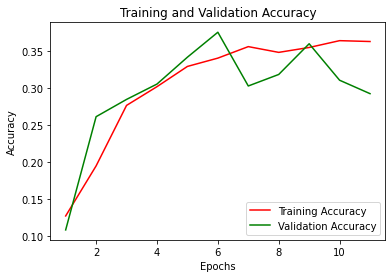
\includegraphics[width=0.9\linewidth]{img/resnet101v2/resnet101feacc.png} 
		\caption{ResNet101V2 Feature Extraction Accuracy}
		\label{fig:resnet101feacc}
	\end{subfigure}
	\begin{subfigure}{0.5\textwidth}
		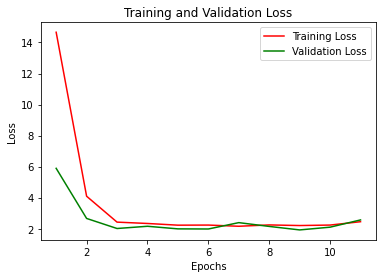
\includegraphics[width=0.9\linewidth]{img/resnet101v2/resnet101feloss.png}
		\caption{ResNet101V2 T Feature Extraction Loss}
		\label{fig:resnet101feloss}
	\end{subfigure}
\end{figure}

The network under-fitted our training, performing drastically poorly. The same considerations done in chapter 4.2.1 apply here.


\subsubsection{Test 2: Finetuning One Sub-Block}
As done for ResNet50, we tried to improve our ResNet101 performance using finetuning. In this paragraph we just finetuned the last sub-block of the network.

\medskip

\begin{tabular}{ |p{2cm}|p{2cm}|p{2cm}|p{2cm}|p{2cm}|  }
\hline
\multicolumn{5}{|c|}{Finetuning One Sub-Block} \\
\hline
\textbf{Epoch stopped} & \textbf{Validation Accuracy} & \textbf{Testing Accuracy} & \textbf{Validation Loss} & \textbf{Testing Loss} \\
\hline
18 & 0.5492 & 0.5218 & 1.7628 & 2.3036\\
\hline
\end{tabular}

\begin{figure}[H]
	\begin{subfigure}{0.5\textwidth}
		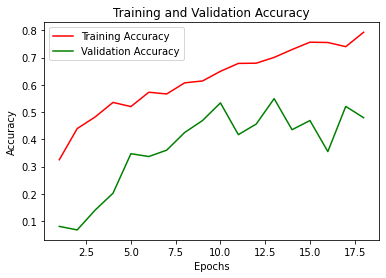
\includegraphics[width=0.9\linewidth]{img/resnet101v2/resnet101ft1acc.png} 
		\caption{ResNet101V2 Test 2 Accuracy}
		\label{fig:resnet101ft1acc}
	\end{subfigure}
	\begin{subfigure}{0.5\textwidth}
		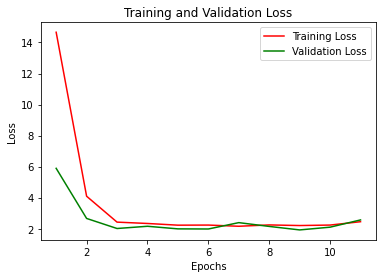
\includegraphics[width=0.9\linewidth]{img/resnet101v2/resnet101feloss.png}
		\caption{ResNet101V2 Test 2 Loss}
		\label{fig:resnet101ft1loss}
	\end{subfigure}
\end{figure}

As expected, the performance are better compered to test 1. Anyway, the network still do not overfit: finetuning just one sub-block is not enough for a neural network made of 101 layers. 

\subsubsection{Test 3: Finetuning the Entire Block 5}
Aiming to overfitting, we finetuned the entire block 5, which is made of 3 sub-blocks.

\medskip

\begin{tabular}{ |p{2cm}|p{2cm}|p{2cm}|p{2cm}|p{2cm}|  }
\hline
\multicolumn{5}{|c|}{Finetuning Entire Block 5} \\
\hline
\textbf{Epoch stopped} & \textbf{Validation Accuracy} & \textbf{Testing Accuracy} & \textbf{Validation Loss} & \textbf{Testing Loss} \\
\hline
15 & 0.5155 & 0.4805 & 1.9216 & 3.4421\\
\hline
\end{tabular}

\begin{figure}[H]
	\begin{subfigure}{0.5\textwidth}
		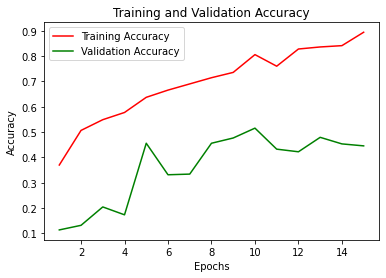
\includegraphics[width=0.9\linewidth]{img/resnet101v2/resnet101ft_block5_acc.png} 
		\caption{ResNet101V2 Test 3 Accuracy}
		\label{fig:resnet101ftblock5acc}
	\end{subfigure}
	\begin{subfigure}{0.5\textwidth}
		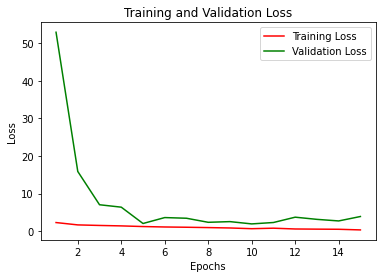
\includegraphics[width=0.9\linewidth]{img/resnet101v2/resnet101ft_block5_loss.png}
		\caption{ResNet101V2 Test 3 Loss}
		\label{fig:resnet101ftblock5loss}
	\end{subfigure}
\end{figure}

Unfortunately, we have little less performance and we still not completely overfitting: the training accuracy is less than 0.9, meaning that we are not finetuning enough but we are following the right lead since the training accuracy gain 0.1 point.


\subsubsection{Test 4: Finetuning Half Block 4}
In this paragraph, heavy finetuning is done setting as trainable parameters all of them after \textit{conv4\_block13\_out} for a total of 13 sub-blocks finetuned (i.e., 10 in block 4 and 3 in block 5).

\medskip

\begin{tabular}{ |p{2cm}|p{2cm}|p{2cm}|p{2cm}|p{2cm}|  }
\hline
\multicolumn{5}{|c|}{Finetuning Half Block 4} \\
\hline
\textbf{Epoch stopped} & \textbf{Validation Accuracy} & \textbf{Testing Accuracy} & \textbf{Validation Loss} & \textbf{Testing Loss} \\
\hline
31 & 0.6114 & 0.5977 & 2.3865 & 2.3642\\
\hline
\end{tabular}

\begin{figure}[H]
	\begin{subfigure}{0.5\textwidth}
		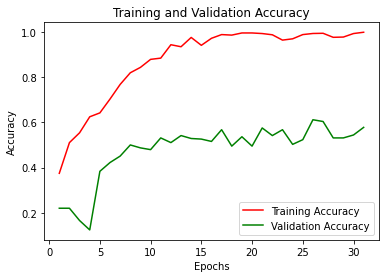
\includegraphics[width=0.9\linewidth]{img/resnet101v2/resnet101ft4acc.png} 
		\caption{ResNet101V2 Test 4 Accuracy}
		\label{fig:resnet101ft4acc}
	\end{subfigure}
	\begin{subfigure}{0.5\textwidth}
		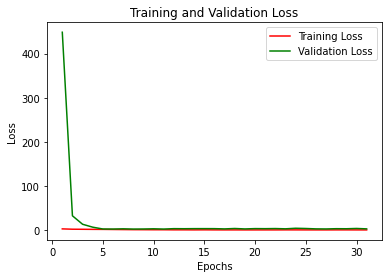
\includegraphics[width=0.9\linewidth]{img/resnet101v2/resnet101ft4loss.png}
		\caption{ResNet101V2 Test 4 Loss}
		\label{fig:resnet101ft4loss}
	\end{subfigure}
\end{figure}

Finetuning these many layers helped the network to be more our topic-specific. In fact, the neural network finally overfit properly our training data as the accuracy plot shows, also even the loss is lesser than before. However, even if we improve from the previous test it is not enough if we consider the best result obtained using ResNet50 or VGG16.


\subsubsection{Test 5: Test 4 and Dropout}
In test 4 the network overfitted, even if not much, we try to use dropout to mitigate this problem. This approach can result in two possible outcomes:

\begin{enumerate}
	\item We perform more or less the same as in test 4: this is the goal of dropout, neutralize neurons but performing the same as before, reducing in this way the number of computations and performing better on the test set.
	\item We perform worst than test 4: dropout neutralizes too many units, performing worst both on the validation set and the test set. This is a problem, the dropout rate should be reduced or other regularization techniques apply.
\end{enumerate}

\noindent The results obtained are the following:

\medskip

\begin{tabular}{ |p{2cm}|p{2cm}|p{2cm}|p{2cm}|p{2cm}|  }
\hline
\multicolumn{5}{|c|}{Finetuning Half Block 4 and Dropout} \\
\hline
\textbf{Epoch stopped} & \textbf{Validation Accuracy} & \textbf{Testing Accuracy} & \textbf{Validation Loss} & \textbf{Testing Loss} \\
\hline
28 & 0.5959 & 0.5356 & 2.2455 & 2.8590\\
\hline
\end{tabular}

\begin{figure}[H]
	\begin{subfigure}{0.5\textwidth}
		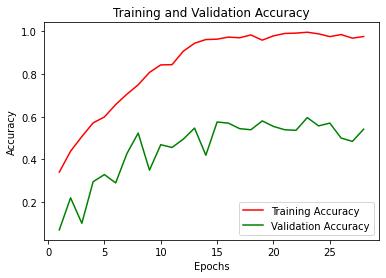
\includegraphics[width=0.9\linewidth]{img/resnet101v2/resnet101ft4_drop_acc.png} 
		\caption{ResNet101V2 Test 5 Accuracy}
		\label{fig:resnet101ft4dropacc}
	\end{subfigure}
	\begin{subfigure}{0.5\textwidth}
		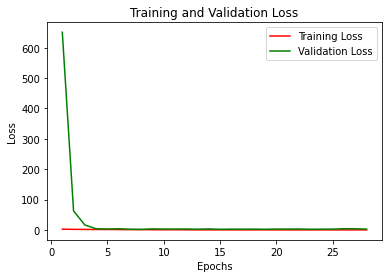
\includegraphics[width=0.9\linewidth]{img/resnet101v2/resnet101ft4_drop_loss.png}
		\caption{ResNet101V2 Test 5 Loss}
		\label{fig:resnet101ft4droploss}
	\end{subfigure}
\end{figure}

The plots and the table show that the situation this test inclines is the second outcome presented. Even if the validation accuracy losses just 0.2 points, the test accuracy has a gap 0.6 points with the one obtained in test 4, which is a lot considering that the overall performance is not good (it barely arrives to 0.6, which is very low to be considered a good classifier). Hence, for the following test we decided to drop the use of dropout until better performances are met.



\subsubsection{Test 6: Adding Dense Layers to Test 4}
Following the tests performed with VGG16 and ResNet50V2, we tried also here to add dense layers at the top of the \textit{GlobalAveragePooling2D} layer.  Doing this experiment, the learning rate of \textit{Adam} is change from the default value (i.e, 0.001) to 0.0001.

\noindent The result obtained are the following:

\medskip

\begin{tabular}{ |p{2cm}|p{2cm}|p{2cm}|p{2cm}|p{2cm}|  }
\hline
\multicolumn{5}{|c|}{Finetuning Half Block 4 and Adding 2 Dense Layers} \\
\hline
\textbf{Epoch stopped} & \textbf{Validation Accuracy} & \textbf{Testing Accuracy} & \textbf{Validation Loss} & \textbf{Testing Loss} \\
\hline
16 & 0.6062 & 0.4552 & 1.6339 & 3.5964\\
\hline
\end{tabular}

\begin{figure}[H]
	\begin{subfigure}{0.5\textwidth}
		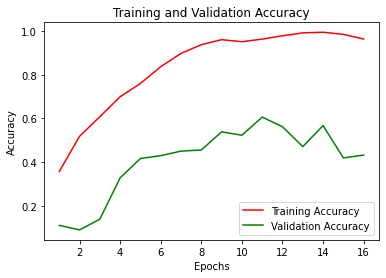
\includegraphics[width=0.9\linewidth]{img/resnet101v2/resnet101ft4denseacc.png} 
		\caption{ResNet101V2 Test 6 Accuracy}
		\label{fig:resnet101ft4denseacc}
	\end{subfigure}
	\begin{subfigure}{0.5\textwidth}
		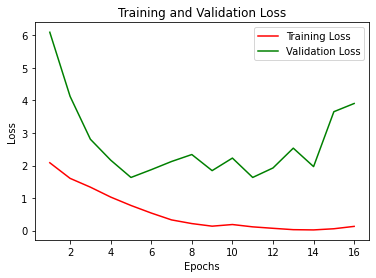
\includegraphics[width=0.9\linewidth]{img/resnet101v2/resnet101ft4denseloss.png}
		\caption{ResNet101V2 Test 6 Loss}
		\label{fig:resnet101ft4denseloss}
	\end{subfigure}
\end{figure}

The introduction of these layers worsen the performance of test 4, but they helped achieving better loss values. Anyway, they had a bad effect on the test accuracy which is now one of the lower values obtained for ResNet101. This can be explained, perhaps, since the network now shrinks in two layers before predicting: layers specialized on the training set. Hence, they ended up discovering features that are not helpful for predicting correctly the test set.


\subsubsection{Test 7: Going Deeper and Deeper}
Since increasing the finetuning level led to better result in the previous tests, we finetuned ResNet101 till \textit{conv3\_block4\_out} including the parameters of all conv4 (i.e., block4). The network in this way has really unbalanced in terms of trainable parameters, most of them were trainable (i.e., about 80\%). Even that, we tested it and what we obtain was a failure, the network didn't learn well an ended up with a tremendous low accuracy. Thus, we decided to limit our going deeper to the \textit{conv4\_block10\_out}: adding three more sub-blocks to the ones tested in test 3 (which is still our current optimum).
\noindent The result obtained are the following:

\medskip

\begin{tabular}{ |p{2cm}|p{2cm}|p{2cm}|p{2cm}|p{2cm}|  }
\hline
\multicolumn{5}{|c|}{Finetuning till conv4\_block10\_ou} \\
\hline
\textbf{Epoch stopped} & \textbf{Validation Accuracy} & \textbf{Testing Accuracy} & \textbf{Validation Loss} & \textbf{Testing Loss} \\
\hline
22 & 0.6062 & 0.5310 & 2.1705 & 2.5997\\
\hline
\end{tabular}

\begin{figure}[H]
	\begin{subfigure}{0.5\textwidth}
		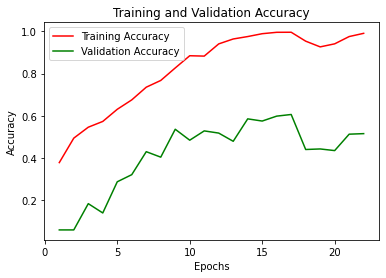
\includegraphics[width=0.9\linewidth]{img/resnet101v2/resnet101ftdeeperacc.png} 
		\caption{ResNet101V2 Test 7 Accuracy}
		\label{fig:resnet101ftdeeperacc}
	\end{subfigure}
	\begin{subfigure}{0.5\textwidth}
		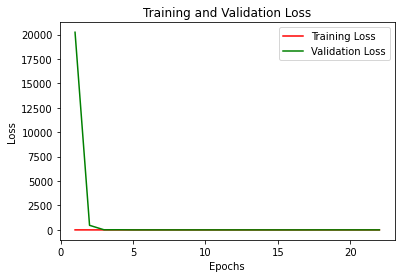
\includegraphics[width=0.9\linewidth]{img/resnet101v2/resnet101ftdeeperloss.png}
		\caption{ResNet101V2 Test 7 Loss}
		\label{fig:resnet101ftdeeperloss}
	\end{subfigure}
\end{figure}

These results gained the second best position for our ResNet101 tests. Anyway, the performance are still too poor and the computational power required for training is very high (i.e., we have about 30M parameters). It is important to notice that the same result for validation was obtained in test 6, but with a lower score for the test accuracy. This indicates that the point is a pitfall, where our validation gets caught and wherever it moves it finds only worst values.
Anyway, we have no way to escape it: the accuracy for the training set is curvilinear without frequent zig-zags, thus changing the learning rate of Adam will let to worst or the same result:
\begin{enumerate}
\item if we decrease the learning rate we increase the possibility to stop earlier or to fall in the same pitfall;
\item if we increase the learning rate we will overfit very fast jeopardizing the training.
\end{enumerate}


\subsection{InceptionV3}

\subsubsection{Test 1: Classical ResNet101V2 with 50 classes}

\subsubsection{Test 2: Completely Newly Output Layers Architecture}

\subsubsection{Test 3: Fine Tuning with One Layer}

\subsubsection{Test 4: Fine Tuning with Two Layers}


